\documentclass[11pt]{article}

\usepackage[a4paper,margin=1in]{geometry}
\usepackage[T1]{fontenc}
\usepackage[utf8]{inputenc}
\usepackage{lmodern}
\usepackage{amsmath}
\usepackage{booktabs}
\usepackage{graphicx}
\usepackage{float}
\usepackage{array}
\usepackage{longtable}
\usepackage{caption}
\usepackage{subcaption}
\usepackage{hyperref}

\title{EC581 HW1\\BIST100 Trend-Following, Mean-Reversion, and Hybrid Strategies}
\author{Hayrettin Akgüç \\ Student ID: 2020300168}
\date{March 27, 2026}

\begin{document}

\maketitle

\begin{center}
\href{https://github.com/haeiau1/EC581}{GitHub Repository: github.com/haeiau1/EC581}
\end{center}

\section{Strategies}
In this homework, I started with the two strategies requested in the assignment. I kept the rules simple at first so that I could clearly see what each idea was doing.

\subsection{Trend Following}
For trend following, I used a simple rule: buy after $n$ consecutive days of positive daily returns and exit after $m$ consecutive days of negative daily returns.

\subsection{Mean Reversion}
For mean reversion, I used the opposite logic: buy after $n$ consecutive days of negative daily returns and exit after $m$ consecutive days of positive daily returns.

\section{Results Before Optimization}
Before doing any optimization, I first tested the strategies with manually chosen parameters. I wanted to see how sensitive the results were, so I looked at two sample periods: a shorter recent sample starting in 2024 and a long sample starting in 1997.

\subsection{Short Sample: 2024--2026}
\begin{table}[H]
\centering
\caption{Manual Results for the 2024--2026 Sample}
\label{tab:manual_2024}
\makebox[\textwidth][c]{%
\resizebox{\textwidth}{!}{%
\begin{tabular}{>{\raggedright\arraybackslash}p{3.8cm}lrrrrrr}
\toprule
Strategy & Parameters & Total Return (\%) & Annual Return (\%) & Volatility (\%) & Sharpe & Max DD (\%) & Trades \\
\midrule
Trend Following & $n=3,\;m=2$ & -9.89 & -4.37 & 11.34 & -0.0212 & 29.99 & 32 \\
Mean Reversion & $n=4,\;m=1$ & 7.36 & 3.38 & 6.64 & 0.0337 & 10.96 & 14 \\
\bottomrule
\end{tabular}
\par}}
\end{table}

In the short sample, I saw the opposite of what later appeared in the long sample. The manually chosen trend-following rule gave a negative return, while the manually chosen mean-reversion rule stayed slightly profitable and also had lower volatility and lower drawdown.

\subsection{Long Sample: 1997--2026}
\begin{table}[H]
\centering
\caption{Manual Results for the 1997--2026 Sample}
\label{tab:manual_1997}
\makebox[\textwidth][c]{%
\resizebox{\textwidth}{!}{%
\begin{tabular}{>{\raggedright\arraybackslash}p{3.8cm}lrrrrrr}
\toprule
Strategy & Parameters & Total Return (\%) & Annual Return (\%) & Volatility (\%) & Sharpe & Max DD (\%) & Trades \\
\midrule
Trend Following & $n=3,\;m=2$ & 361.16 & 13.52 & 18.17 & 0.0496 & 38.55 & 378 \\
Mean Reversion & $n=4,\;m=1$ & -7.53 & -0.26 & 10.52 & 0.0017 & 34.93 & 183 \\
\bottomrule
\end{tabular}
\par}}
\end{table}

When I moved to the long sample, the picture changed. Trend following produced positive performance, while the manually selected mean-reversion rule did not generate meaningful returns.

\begin{figure}[H]
\centering

\includegraphics[width=0.9\textwidth]{output/start_1997-07-01__end_2026-03-27__trend_n3_m2__mean_n4_m1/equity_curves.png}
\caption{Manual baseline equity curves for the long sample.}
\label{fig:manual_equity}
\end{figure}

\section{Optimization of the Two Assignment Strategies}
After that, I optimized both strategies over all $n,m \in \{1,\dots,10\}$. I used Sharpe ratio as the main selection criterion because I wanted to compare return together with risk.

\begin{table}[H]
\centering
\caption{Optimized Trend Following and Mean Reversion}
\label{tab:optimized_classic}
\makebox[\textwidth][c]{%
\resizebox{\textwidth}{!}{%
\begin{tabular}{>{\raggedright\arraybackslash}p{3.8cm}lrrrrrr}
\toprule
Strategy & Best Parameters & Total Return (\%) & Annual Return (\%) & Volatility (\%) & Sharpe & Max DD (\%) & Trades \\
\midrule
Trend Following & $n=4,\;m=6$ & 605.80 & 23.70 & 28.85 & 0.0555 & 68.86 & 26 \\
Mean Reversion & $n=1,\;m=10$ & 637.40 & 25.08 & 33.41 & 0.0527 & 62.97 & 17 \\
\bottomrule
\end{tabular}
\par}}
\end{table}

After optimization, the gap between the two strategies became much smaller. Trend following ended up with a slightly higher Sharpe ratio, while mean reversion ended up with a slightly higher total return. This made me think that both ideas are capturing something real in BIST100, and that the earlier difference was partly driven by the initial parameter choice.

\section{Motivation for the Hybrid Strategy}
Since the optimized trend-following and mean-reversion results were quite close, my next thought was to see whether I could combine the two ideas. That is why I introduced a hybrid strategy.

The idea was the following:
\begin{itemize}
    \item first use a long-term trend filter to decide whether the market is in an upward regime,
    \item then apply a mean-reversion type entry rule only inside that positive trend regime.
\end{itemize}

Formally, the regime filter is:
\[
\text{Close}_t > \text{SMA}_{L}(t)
\]
where $L$ is the long-term trend period.

So the hybrid rule becomes:
\begin{itemize}
    \item Buy after $n$ consecutive negative return days, but only if price is above the long-term moving average.
    \item Exit after $m$ consecutive days with price below the same long-term moving average.
\end{itemize}

My goal here was to combine the direction filter of trend following with the entry timing idea of mean reversion.

\section{Hybrid Strategy Before Optimization}
I first tested the hybrid strategy with a manually chosen specification.

\begin{table}[H]
\centering
\caption{Manual Hybrid Strategy}
\label{tab:manual_hybrid}
\makebox[\textwidth][c]{%
\resizebox{\textwidth}{!}{%
\begin{tabular}{>{\raggedright\arraybackslash}p{4.4cm}lrrrrrr}
\toprule
Strategy & Parameters & Total Return (\%) & Annual Return (\%) & Volatility (\%) & Sharpe & Max DD (\%) & Trades \\
\midrule
Hybrid Strategy & $n=3,\;m=2,\;L=200$ & 378.26 & 14.20 & 22.03 & 0.0449 & 59.52 & 33 \\
\bottomrule
\end{tabular}
\par}}
\end{table}

This manual hybrid version improved total return relative to the manual trend-following setup, but its Sharpe ratio was still low. So at this point I did not see it as clearly better yet.

\section{Hybrid Optimization Without Trend-Period Search}
As a next step, I optimized the hybrid strategy while keeping the long-term filter fixed at $L=200$. In this version, I only searched over $n$ and $m$.

\begin{table}[H]
\centering
\caption{Hybrid Optimization with Fixed Trend Period}
\label{tab:hybrid_fixed}
\makebox[\textwidth][c]{%
\resizebox{\textwidth}{!}{%
\begin{tabular}{>{\raggedright\arraybackslash}p{4.4cm}lrrrrrr}
\toprule
Strategy & Best Parameters & Total Return (\%) & Annual Return (\%) & Volatility (\%) & Sharpe & Max DD (\%) & Trades \\
\midrule
Hybrid Strategy & $n=4,\;m=6,\;L=200$ & 377.49 & 14.17 & 21.49 & 0.0456 & 49.86 & 20 \\
\bottomrule
\end{tabular}
\par}}
\end{table}

With a fixed long-term filter, the hybrid strategy became a bit more stable and drawdown improved. Still, it did not beat the optimized versions of the two original strategies in Sharpe terms.

\section{Hybrid Optimization With Trend-Period Search}
Finally, I also let the trend period change and optimized the hybrid strategy over three dimensions:
\[
n,\;m,\;L
\]
with $n,m \in \{1,\dots,10\}$ and $L \in \{50,100,150,200\}$.

\begin{table}[H]
\centering
\caption{Hybrid Optimization with Trend-Period Search}
\label{tab:hybrid_full}
\makebox[\textwidth][c]{%
\resizebox{\textwidth}{!}{%
\begin{tabular}{>{\raggedright\arraybackslash}p{4.4cm}lrrrrrr}
\toprule
Strategy & Best Parameters & Total Return (\%) & Annual Return (\%) & Volatility (\%) & Sharpe & Max DD (\%) & Trades \\
\midrule
Hybrid Strategy & $n=1,\;m=4,\;L=100$ & 541.96 & 20.96 & 24.44 & 0.0567 & 42.67 & 58 \\
\bottomrule
\end{tabular}
\par}}
\end{table}

This turned out to be the best active hybrid result in the project. Once I allowed the long-term filter to vary, the hybrid strategy achieved the highest Sharpe ratio among the active strategies I tested, and it also had a lower maximum drawdown than the optimized baseline strategies.

\begin{figure}[H]
\centering
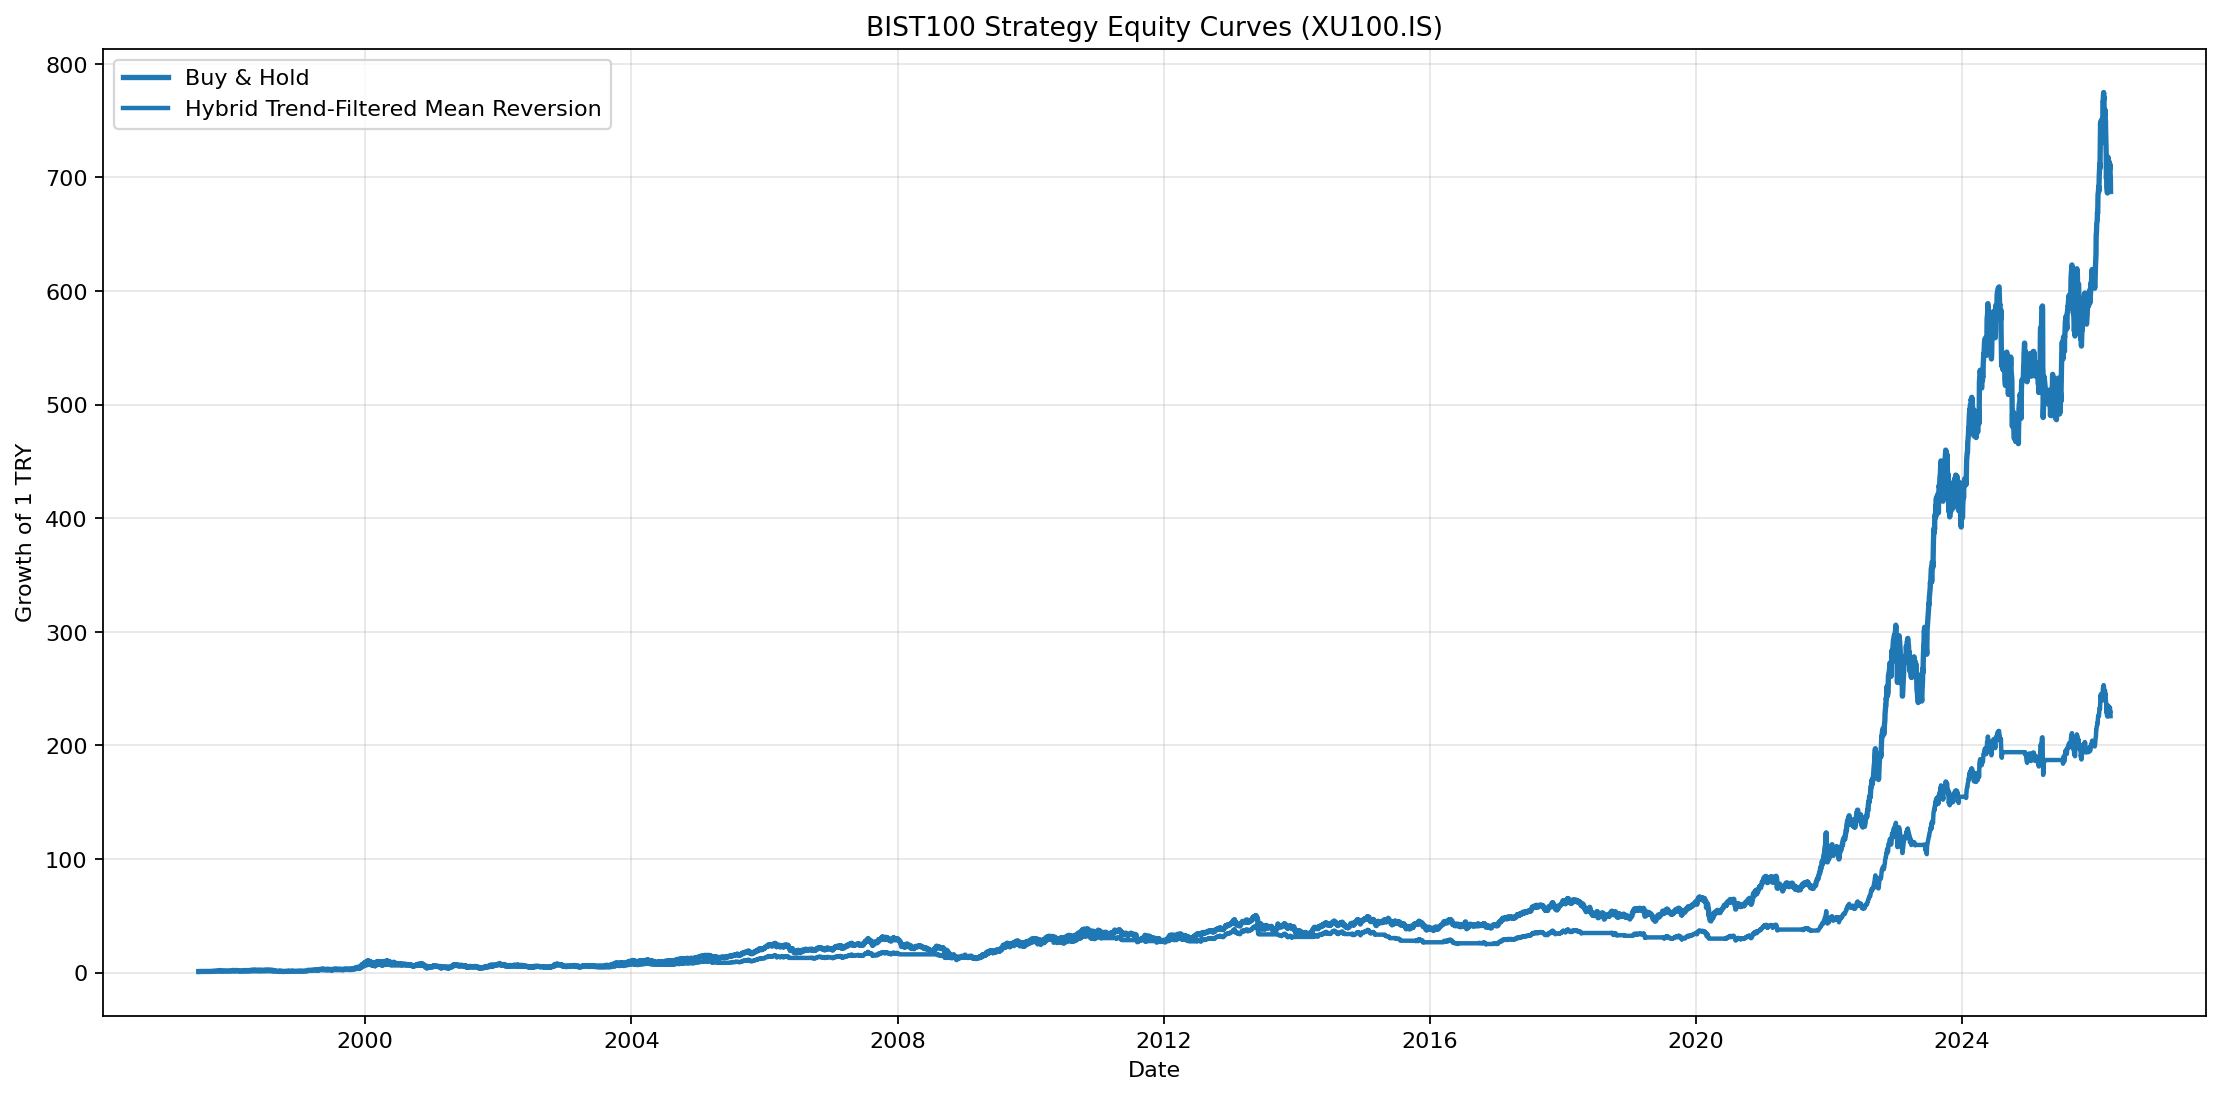
\includegraphics[width=0.9\textwidth]{output/hybrid__start_1997-07-01__end_2026-03-27__n1__m4__trend100/equity_curves.png}
\caption{Equity curve of the final hybrid configuration ($n=1$, $m=4$, $L=100$).}
\label{fig:hybrid_equity}
\end{figure}

\section{All Results in One Table}
In Table~\ref{tab:all_results}, I collected all of the main configurations, both optimized and non-optimized, in one place so that the comparison is easier to see.

\begin{table}[H]
\centering
\caption{Full Comparison of All Main Results}
\label{tab:all_results}
\makebox[\textwidth][c]{%
\resizebox{\textwidth}{!}{%
\begin{tabular}{>{\raggedright\arraybackslash}p{5.0cm}lrrrrrr}
\toprule
Version & Parameters & Total Return (\%) & Annual Return (\%) & Volatility (\%) & Sharpe & Max DD (\%) & Trades \\
\midrule
Trend Following, manual (1997--2026) & $n=3,\;m=2$ & 361.16 & 13.52 & 18.17 & 0.0496 & 38.55 & 378 \\
Mean Reversion, manual (1997--2026) & $n=4,\;m=1$ & -7.53 & -0.26 & 10.52 & 0.0017 & 34.93 & 183 \\
Trend Following, optimized & $n=4,\;m=6$ & 605.80 & 23.70 & 28.85 & 0.0555 & 68.86 & 26 \\
Mean Reversion, optimized & $n=1,\;m=10$ & 637.40 & 25.08 & 33.41 & 0.0527 & 62.97 & 17 \\
Hybrid, manual & $n=3,\;m=2,\;L=200$ & 378.26 & 14.20 & 22.03 & 0.0449 & 59.52 & 33 \\
Hybrid, optimized with fixed $L$ & $n=4,\;m=6,\;L=200$ & 377.49 & 14.17 & 21.49 & 0.0456 & 49.86 & 20 \\
Hybrid, optimized with variable $L$ & $n=1,\;m=4,\;L=100$ & 541.96 & 20.96 & 24.44 & 0.0567 & 42.67 & 58 \\
Buy \& Hold benchmark & --- & 68657.97 & 25.78 & 34.76 & 0.7417 & 63.43 & 0 \\
\bottomrule
\end{tabular}
\par}}
\end{table}

\section{Conclusion}
My main takeaway is that the first impression depends a lot on parameter choice and sample period. With the manual parameter choices, trend following looked much stronger than mean reversion in the long sample, but not in the short sample. After optimization, the two strategies became much closer. Trend following was slightly better in Sharpe ratio, while mean reversion was slightly better in total return.

Because of that, I thought it made sense to try a combined approach instead of choosing only one side. The hybrid strategy was my attempt to do that by using a trend filter together with a pullback-style entry rule. When the trend period was fixed, the hybrid strategy improved drawdown but still was not clearly the best. When I optimized the trend period as well, the hybrid strategy gave the best Sharpe ratio among the active strategies.

So, if I only compare the two original assignment strategies, I would say trend following looks slightly better on a risk-adjusted basis. But if I allow myself to combine the two ideas, then the hybrid strategy with $L=100$, $n=1$, and $m=4$ looks like the most attractive active version in this homework.

At the same time, the buy-and-hold benchmark is still much stronger than all of the active strategies in total performance and Sharpe ratio. So my final conclusion is that these simple trading rules do show some structure, but they are not strong enough to beat passive long-run exposure to BIST100 over the full sample.

\end{document}
